\documentclass{acmart}

\title{Example Paper Title}
\author{Paul Tarvydas}
\affiliation{%
  \institution{retired}
  \city{Toronto}
  \state{Ontario}
  \country{Canada}
}
\email{ptarvydas@institution1.edu}

\author{Zac Nowicki}
\affiliation{%
  \institution{Kagi}
  \city{Palo Alto}
  \state{CA}
  \country{USA}
}
\email{znowicki@institution2.edu}

\begin{document}

\maketitle

\begin{figure}[h]
  \centering
  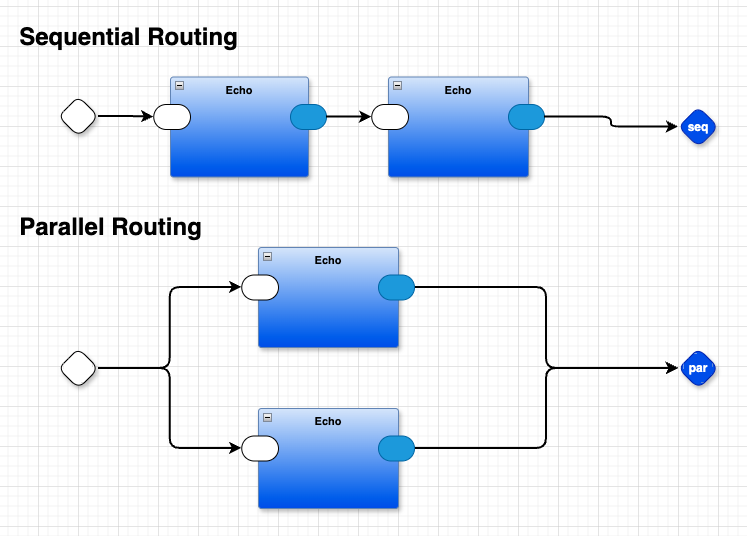
\includegraphics[width=0.5\linewidth]{HelloWorld0D.png}
  \caption{Motivating Example for a DPL}
  \label{fig:example}
\end{figure}

The above diagram is a motivating example.

The above diagram shows but one sample of a practical DPL syntax. Variations and improvements on this syntax can be imagined. The above syntax is being used to produce actual applications like term-rewriting (t2t text-to-text rewriting) compilers, LLMs, DSLs for creating DSLs, Visual Shell prototypes, games, etc.

This DPL syntax consists of only a few kinds of closed figures plus arrows plus text belonging to the closed figures. Everything else is considered to be a comment and is ignored. For example, the bold text “Sequential Routing” is ignored. Colors are ignored. Line shapes and line widths are ignored, and so on.

This diagram was drawn using the off-the-shelf diagram editor draw.io\footnote{\url{https://www.draw.io}}. The editor saves the diagram in a modified form of XML, called graphML\footnote{\url{https://en.wikipedia.org/wiki/GraphML}}.

\end{document}
